\begin{figure}[tb]
    \centering
    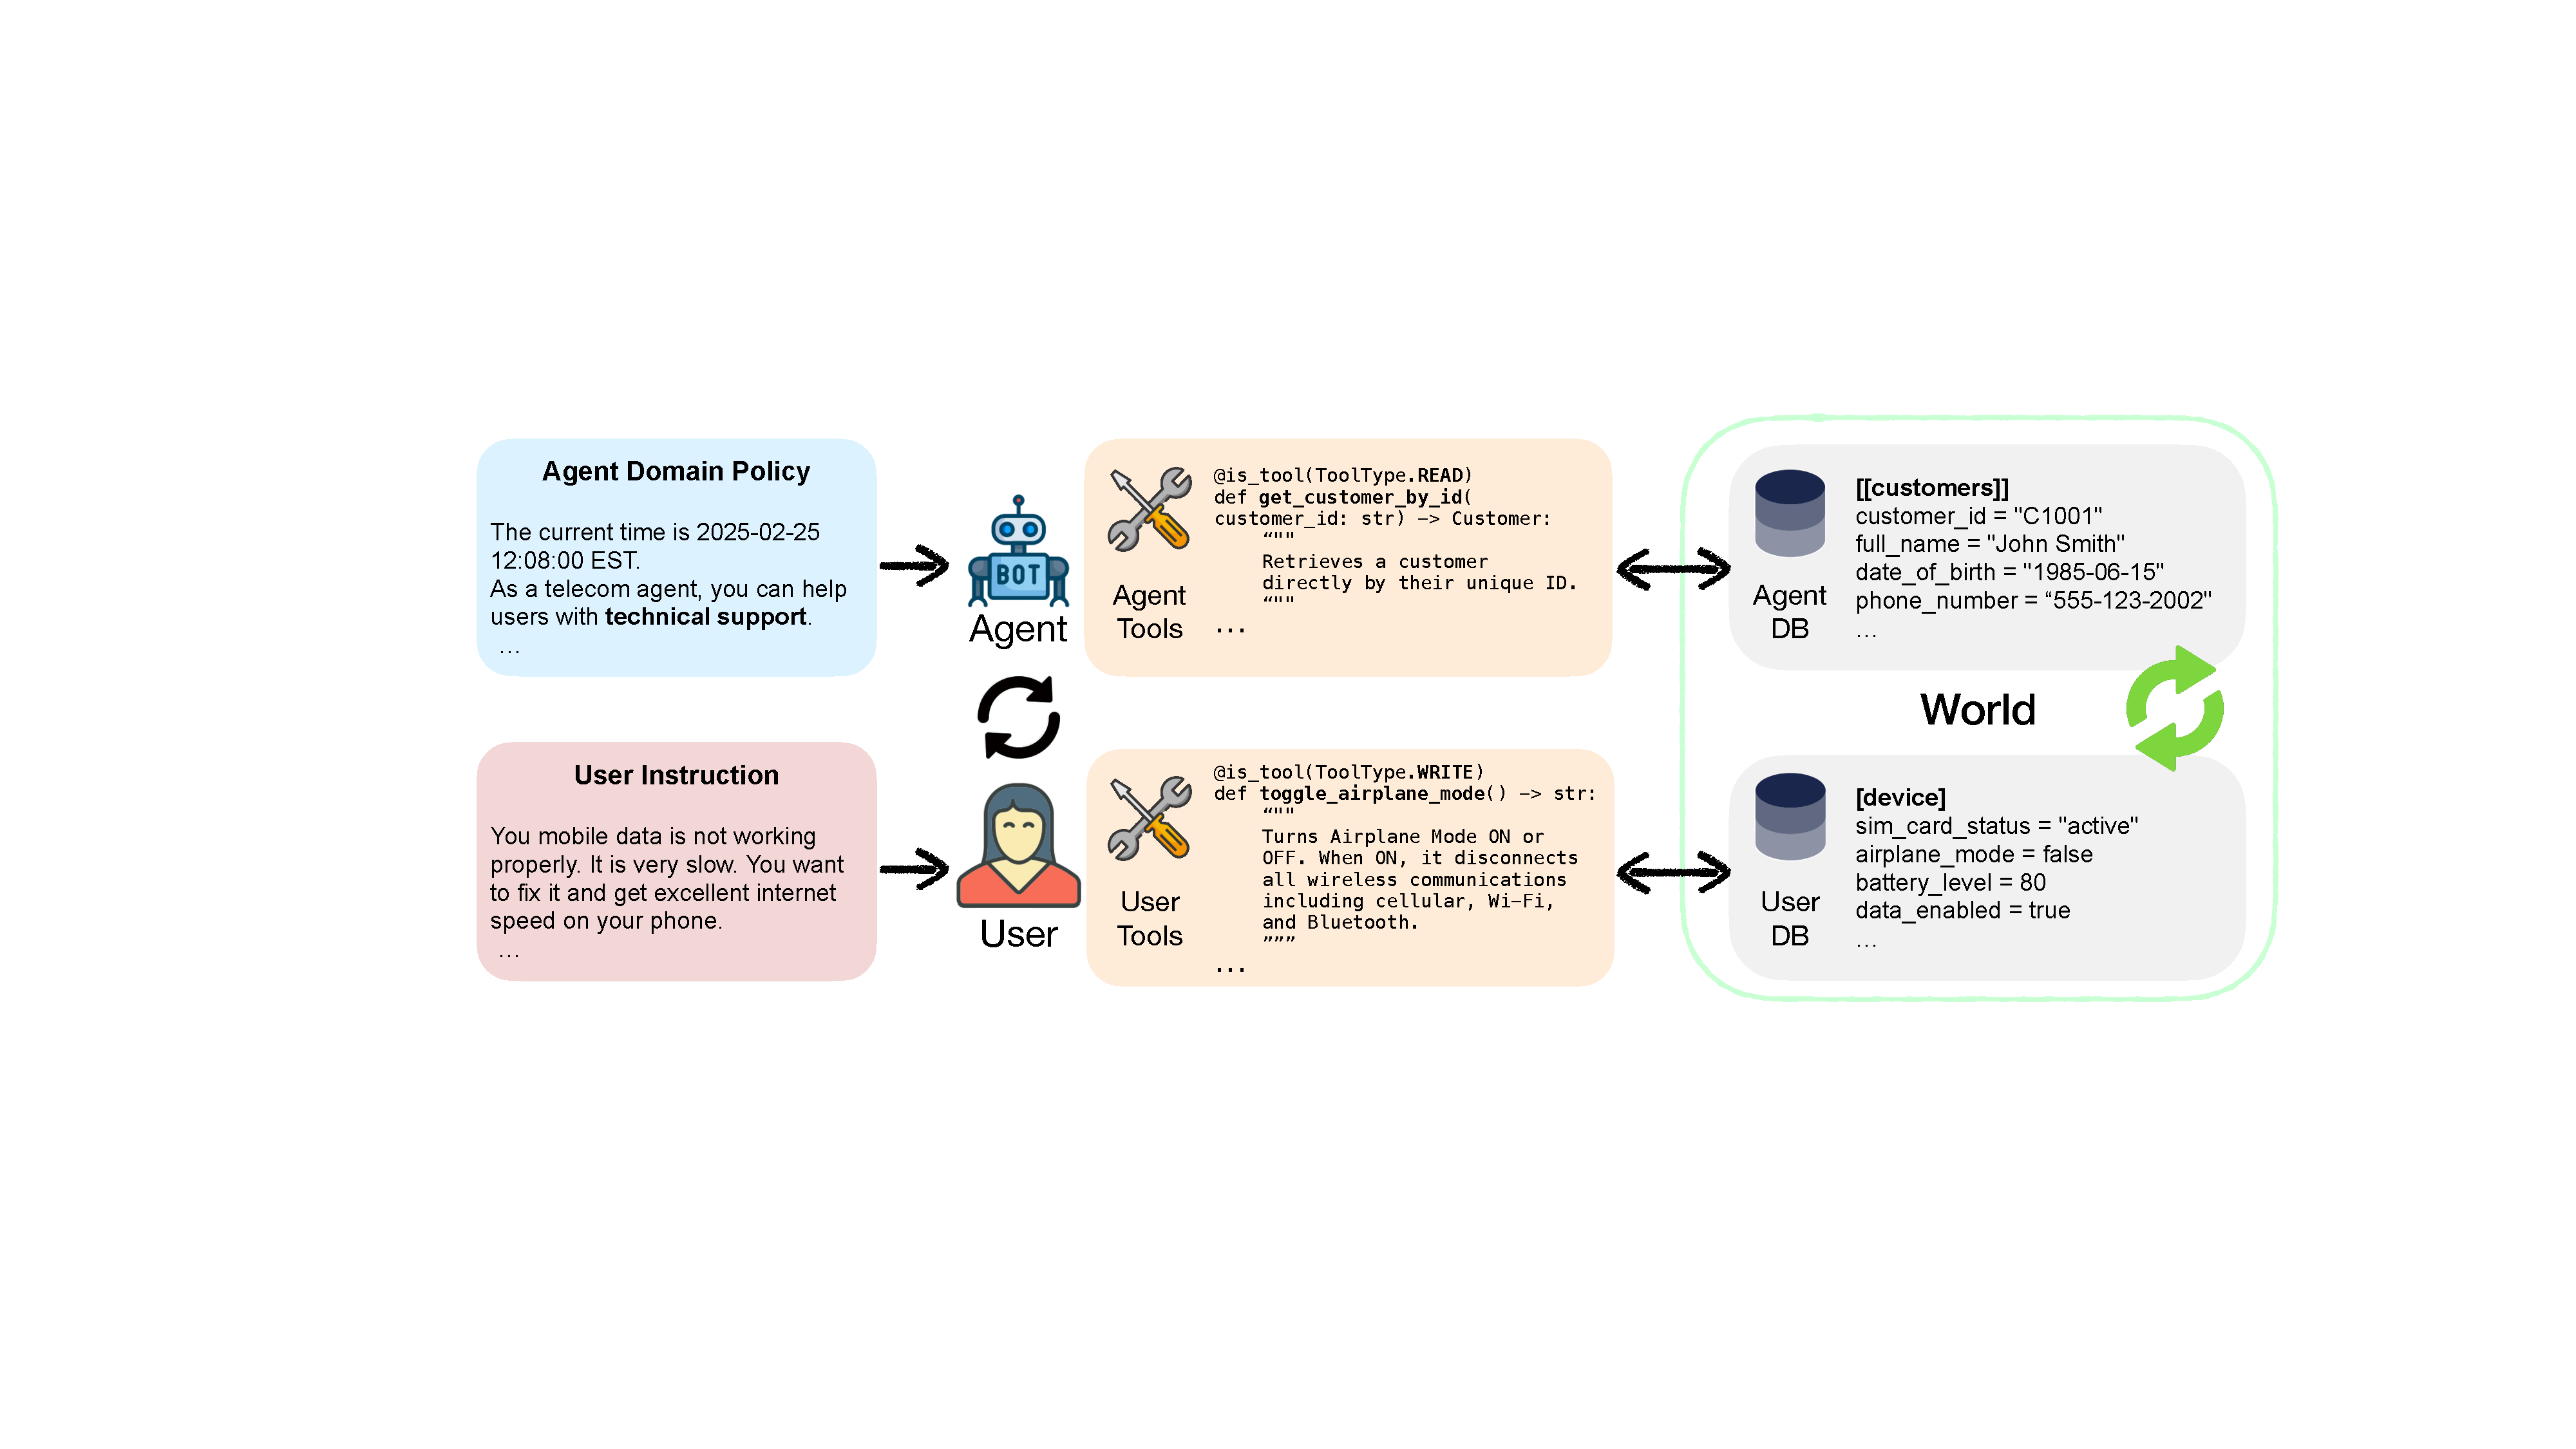
\includegraphics[width=0.99\textwidth,trim=340 330 220 300,clip]{figures/raw/teaser.pdf}
    \vspace{-0.5em}
    \caption{Supporting dual-control environment in \bench. The agent have access to a set of tools that interact with a database, and is tasked with resolving the user's request via Tool-Agent-User (TAU) interactions while adhering to the domain policy. To test real-world scenarios, the user is simulated by another AI agent given a scenario-based instruction and a set of tools that interact with its own database. The simulated user can be regarded as handling an easier version of the TAU interaction in a dual format (Tool-User-Agent), where it only need to follow instructions but does not need to reason about solutions for the task.}
    \label{fig:teaser}
\end{figure}

